\documentclass[border=10pt]{standalone}
\usepackage[svgnames]{xcolor}
\usepackage{amsmath}
\usepackage{pgfplots}
\pgfplotsset{compat=newest}
\usepackage[sfdefault]{FiraSans}
\usepackage{FiraMono}
\renewcommand*\familydefault{\sfdefault}
\begin{document}
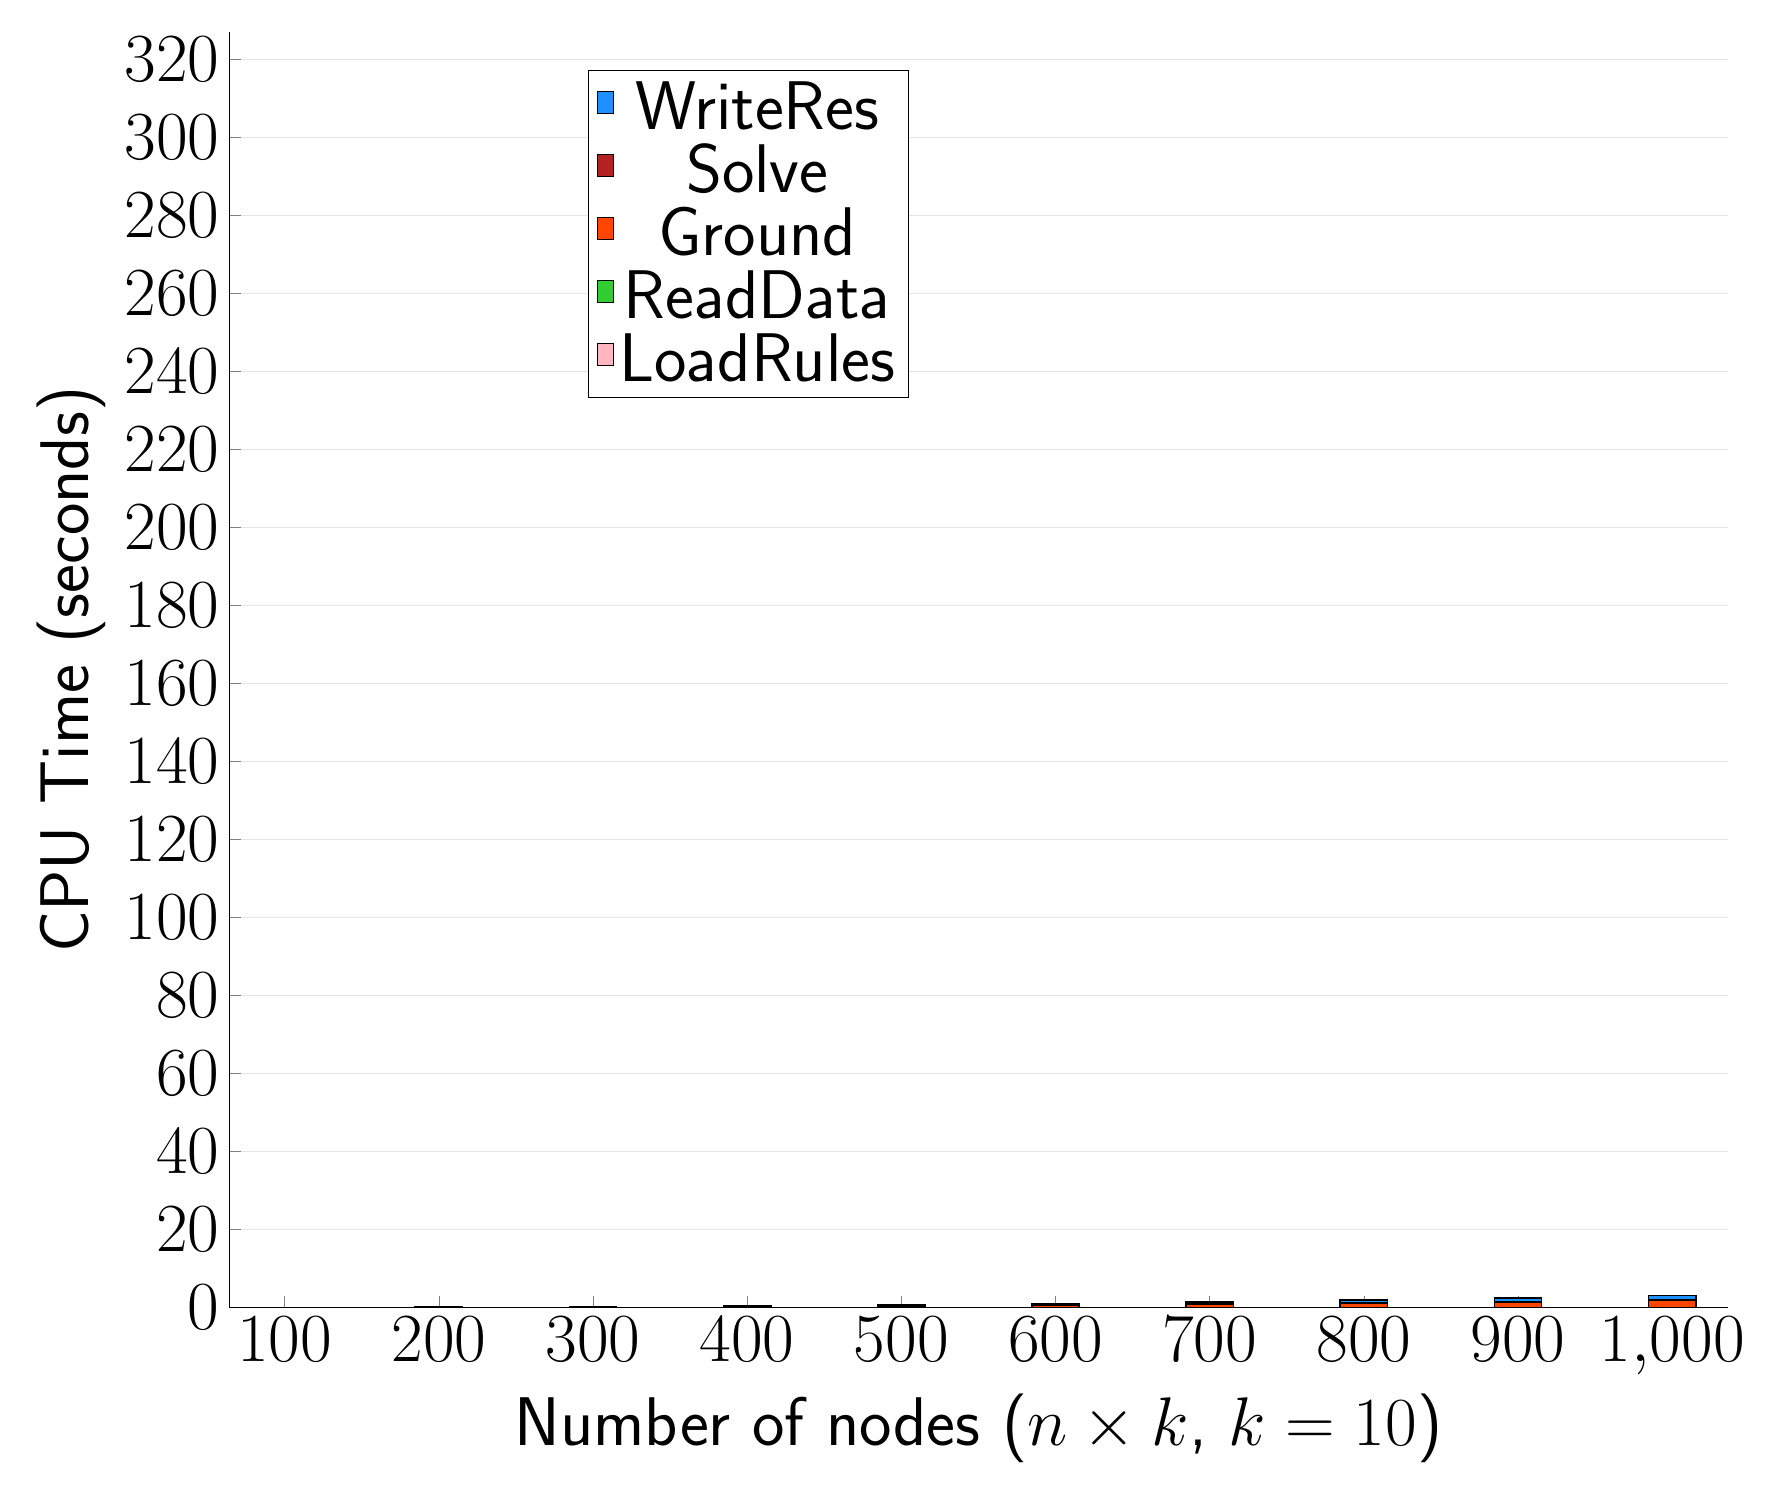
\begin{tikzpicture}
\begin{axis}[
   ybar stacked,
   width=1.7\textwidth,
   bar width=0.6cm,
   ymajorgrids, tick align=inside,
   major grid style={draw=gray!20},
   xtick=data,
   ymin=0, ymax=326.9108,
   axis x line*=bottom,
   axis y line*=left,
   enlarge x limits=0.04,
   legend style={
       at={(0.454, 0.97)},
       anchor=north east,
       legend columns=1,
       font=\Huge,
   },
   ylabel={CPU Time (seconds)},
   xlabel={Number of nodes ($n \times k$, $k=10$)},
   label style={font=\Huge},
   tick label style={font=\Huge},
]
\addlegendimage{fill=DodgerBlue, draw=black, line width=0.2pt}
\addlegendentry{WriteRes}
\addlegendimage{fill=FireBrick, draw=black, line width=0.2pt}
\addlegendentry{Solve}
\addlegendimage{fill=OrangeRed, draw=black, line width=0.2pt}
\addlegendentry{Ground}
\addlegendimage{fill=LimeGreen, draw=black, line width=0.2pt}
\addlegendentry{ReadData}
\addlegendimage{fill=LightPink, draw=black, line width=0.2pt}
\addlegendentry{LoadRules}
\addplot +[fill=LightPink, draw=black, line width=0.55pt] coordinates {
(100, 0.0)
(200, 0.0)
(300, 0.0)
(400, 0.0)
(500, 0.0)
(600, 0.0)
(700, 0.0)
(800, 0.0)
(900, 0.0)
(1000, 0.0)
};
\addplot +[fill=LimeGreen, draw=black, line width=0.55pt] coordinates {
(100, 0.0)
(200, 0.0020000000000000018)
(300, 0.0020000000000000018)
(400, 0.010000000000000009)
(500, 0.010000000000000009)
(600, 0.010000000000000009)
(700, 0.010000000000000009)
(800, 0.020000000000000018)
(900, 0.020000000000000018)
(1000, 0.020000000000000018)
};
\addplot +[fill=OrangeRed, draw=black, line width=0.55pt] coordinates {
(100, 0.014000000000000012)
(200, 0.06)
(300, 0.14200000000000002)
(400, 0.246)
(500, 0.4040000000000001)
(600, 0.592)
(700, 0.8480000000000001)
(800, 1.098)
(900, 1.4200000000000002)
(1000, 1.7879999999999998)
};
\addplot +[fill=FireBrick, draw=black, line width=0.55pt] coordinates {
(100, 0.0040000000000000036)
(200, 0.006000000000000005)
(300, 0.006000000000000005)
(400, 0.014000000000000007)
(500, 0.014000000000000012)
(600, 0.02200000000000002)
(700, 0.030000000000000034)
(800, 0.04399999999999982)
(900, 0.05400000000000005)
(1000, 0.060000000000000095)
};
\addplot +[fill=DodgerBlue, draw=black, line width=0.55pt] coordinates {
(100, 0.008000000000000007)
(200, 0.04199999999999998)
(300, 0.10599999999999998)
(400, 0.17599999999999996)
(500, 0.2919999999999999)
(600, 0.40800000000000003)
(700, 0.5619999999999999)
(800, 0.7420000000000002)
(900, 0.914)
(1000, 1.154)
};
\end{axis}
\end{tikzpicture}

\end{document}
